% This version of CVPR template is provided by Ming-Ming Cheng.
% Please leave an issue if you found a bug:
% https://github.com/MCG-NKU/CVPR_Template.

\documentclass[final]{cvpr}

\usepackage{times}
\usepackage{epsfig}
\usepackage{graphicx}
\usepackage{amsmath}
\usepackage{amssymb}
\usepackage{float}
\usepackage{overpic}
\usepackage{caption}
\usepackage{booktabs}
\usepackage{multirow}
\usepackage{tikz}
\usetikzlibrary{arrows.meta, positioning, fit, backgrounds}

\usepackage[pagebackref=true,breaklinks=true,colorlinks,bookmarks=false]{hyperref}

\newcommand{\best}[1]{\textbf{#1}}

\begin{document}

%%%%%%%%% TITLE
\title{VulnScout: Tool-Grounded Vulnerability Triage with a Deterministic Core,\\and Fine-Tuning a Small Model to Use It}

\author{Yuanhao Cao\\
MS in Information Systems\\
Northeastern University\\
cao.yuanh@northeastern.edu
}

\twocolumn[{
    \renewcommand\twocolumn[1][]{#1}%
    \maketitle
    \begin{center}
      \centering
      \IfFileExists{fig/webui.png}{%
        \includegraphics[width=\textwidth]{fig/webui.png}%
      }{%
        \fbox{\parbox[c][5.2cm][c]{0.96\textwidth}{\centering\large Screenshot of the web interface (fig/webui.png)}}%
      }
      \captionof{figure}{The VulnScout web interface answering ``Our Java service runs Log4j 2.14.1. What should we fix first?''. Each tool call appears as a collapsible step above the answer, with a one-line summary of its result and the raw JSON, so the user can check what every statement is based on. The answer lists the affecting CVEs in risk order (known-exploited first), links each one to its NVD, KEV or EPSS record, and ends with the upgrade target that fixes all of them.}
      \label{fig_teaser}
    \end{center}
}]

%%%%%%%%% BODY TEXT
\section*{Abstract}
Developers who ask a general-purpose LLM which known vulnerabilities affect a dependency get answers that are dated, version-inexact and hard to verify. VulnScout is a conversational assistant that keeps every vulnerability fact outside the model. A deterministic core gathers candidate CVEs from NVD and OSV, decides whether the user's exact version is affected from three sources in order of reliability (NVD CPE configurations, CNA records, OSV ranges) with provenance and confidence, ranks findings by exploitation evidence (CISA KEV, then EPSS, then CVSS), and computes an upgrade target that fixes all of them. An LLM agent calls this core and four other tools, including retrieval over MITRE CWE and ATT\&CK, and writes a cited answer. We also generate tool-use dialogues from the deterministic core and fine-tune Qwen3-4B with LoRA to drive the same tools. On 119 held-out questions about eight products unseen in training, Claude Opus 5.5 with the tools recalls 99.8\% of affecting CVEs with no unsupported CVE IDs; the same model without tools recalls 61.9\% and names 380 CVEs that do not affect the asked version. Fine-tuning raises Qwen3-4B's recall from 44.1\% to 93.4\% and removes its fabricated IDs, after 1.8 GPU-hours of training.

%-------------------------------------------------------------------------
\section{Introduction}
\label{sec:intro}

Vulnerability management is a daily task for every team that runs software, and its volume keeps growing: NVD published more than 600 CVE records per day in the week before this project started~\cite{nvd}. Teams without dedicated security staff mostly need two answers: \emph{does a vulnerability affect the exact version I run}, and \emph{what should I fix first?} Severity scores do not settle the second question, since only a small fraction of vulnerabilities is ever exploited; signals such as EPSS~\cite{jacobs2019epss,jacobs2023epss} and the CISA Known Exploited Vulnerabilities (KEV) catalog~\cite{cisakev} were created for that reason.

General-purpose LLMs answer such questions fluently but fail in characteristic ways. Their knowledge stops at a training cutoff; they generate version ranges instead of computing them; they tend to rank by severity; and they produce plausible identifiers that are not supported by any record, a failure already documented for software package names~\cite{spracklen2025package}. Software composition analysis scanners~\cite{trivy,grype,osvscanner,dependabot} match versions accurately, but they expect lock files or images, return lists rather than answers, and do not explain or converse.

VulnScout combines the two: the LLM does the language work (understanding the question, choosing tools, explaining the result) and deterministic code does everything that has a right answer (identifying the product, comparing versions, ranking, computing the fix). Phase 1 proposed this design; this report describes the implemented system and evaluates it. Our contributions are:
\begin{enumerate}
  \item A \textbf{deterministic, multi-source vulnerability core} that resolves each candidate CVE against the user's version from NVD CPE configurations, CNA records and OSV ranges, with provenance and confidence, ranks by exploitation evidence and computes an upgrade target by iterating to a fixed point (Section~\ref{sec:contrib}).
  \item A \textbf{tool-grounded agent} with product verification, abstention for missing or unpublished versions and unknown packages, citations, and BM25 retrieval over CWE~\cite{cwe} and ATT\&CK~\cite{attack} for conceptual questions.
  \item A recipe that turns the deterministic core into \textbf{supervised tool-use data}, used to LoRA-fine-tune~\cite{hu2022lora} Qwen3-4B~\cite{qwen3} so that a small local model can run the same agent.
  \item A \textbf{reproducible evaluation} on a frozen data snapshot with held-out products, comparing four backends, plus a separate evaluation of conceptual questions with and without retrieval.
\end{enumerate}
The code, generated data recipe and all evaluation outputs are public~\cite{vulnscoutrepo}.

%-------------------------------------------------------------------------
\section{Related Work}
\label{sec:related}

\textbf{Vulnerability data and prioritization.} NVD~\cite{nvd} enriches CVE records with CVSS scores, CWE weakness types and CPE configurations, which state the affected products and version ranges in machine-readable form. The CVE Program publishes the original CNA-submitted records~\cite{cvelistv5}, and OSV~\cite{osv} provides package-level ranges for open-source ecosystems. EPSS~\cite{jacobs2019epss,jacobs2023epss} estimates the probability of exploitation in the next 30 days, and CISA KEV~\cite{cisakev} lists vulnerabilities with confirmed exploitation. VulnScout uses these sources rather than replacing them.

\textbf{Software composition analysis.} Trivy~\cite{trivy}, Grype~\cite{grype}, OSV-Scanner~\cite{osvscanner} and Dependabot~\cite{dependabot} match dependency manifests against vulnerability databases. They are accurate for structured inputs but do not take free-form questions, explain priorities or support follow-up questions. VulnScout's core performs the same kind of matching and adds the conversational layer.

\textbf{LLMs in cybersecurity.} Surveys~\cite{xu2024llmsecurity} and benchmarks such as CyberMetric~\cite{tihanyi2024cybermetric} and CTIBench~\cite{alam2024ctibench} measure what models \emph{know} about security. Open-source chatbots over NVD exist~\cite{nvdchatbot,cvellmdataset}, but we did not find one that evaluates version correctness against a ground truth. Our evaluation instead measures whether answers are correct for a specific version and supported by retrieved records.

\textbf{Tool use and retrieval.} RAG~\cite{lewis2020rag} conditions generation on retrieved text, and ReAct~\cite{yao2023react} and Toolformer~\cite{schick2023toolformer} interleave reasoning with tool calls. FreshQA~\cite{vu2023freshllms} and RealTime QA~\cite{kasai2022realtimeqa} show that static models fail on fast-changing facts. For conceptual retrieval we use BM25~\cite{robertson2009bm25}, a lexical ranking function.

\textbf{Fine-tuning for tool use.} Gorilla~\cite{patil2023gorilla} and ToolLLM~\cite{qin2024toolllm} fine-tune open models on API-call data generated with a stronger model, and FireAct~\cite{chen2023fireact} fine-tunes agents on trajectories from GPT-4. Our data instead comes from a deterministic program: every tool call and every fact in the target answers is computed, so the labels are correct by construction and no model output is used for training.

%-------------------------------------------------------------------------
\section{Technical Contribution}
\label{sec:contrib}

\textbf{Multi-source version resolution.} For a product and version, the core first collects candidate CVEs: all CVEs NVD links to the product's CPE vendor/product pairs, plus all OSV advisories for its package. It then decides, per CVE, \emph{affected}, \emph{not affected} or \emph{unknown} from three evidence sources in order of reliability: NVD CPE configurations, CNA records~\cite{cvelistv5} (structured \texttt{lessThan} bounds, \texttt{changes} lists, default status, and parsed free-text ranges such as ``2.0.0 through 2.14.1''), and OSV event lists (introduced, fixed, last affected). Versions are compared with ecosystem rules: PEP~440 for PyPI and Maven-style token ordering otherwise, with pre-releases ordered below their release. One rule turned out to matter: NVD encodes a bound such as ``versions from 2.0-beta9'' on the release line, so a pre-release equal to a bound's release is treated as on that bound. Each verdict keeps its source, a human-readable detail and a confidence: high when NVD decides and no source contradicts it, or when two sources agree; medium for a single uncontested source; low when sources disagree or the evidence was parsed from text. When NVD's upper bound is exclusive, that bound is the fix version.

\textbf{Exploitation-aware ranking and upgrade target.} Affected findings are sorted by KEV membership (ransomware use first), then EPSS, then CVSS, and each gets a reason and a tier (patch now, high, medium, low). A single ``fixed in'' version per CVE is not enough to advise an upgrade: upgrading to the highest fix version of the current findings can land on a version affected by \emph{newer} CVEs. The core therefore evaluates the candidate target with the same pipeline and repeats until no affected finding remains or no fix is known (a fixed point, at most five rounds), and reports any CVE the target still does not fix.

\textbf{A verifying, abstaining agent.} The agent never guesses identifiers. It confirms the product with \texttt{search\_cpe} (CPE dictionary search aggregated into vendor/product pairs) and \texttt{check\_package} (deps.dev~\cite{depsdev}: existence, published versions, nearest published versions when the asked one does not exist, PEP~503 name normalization, and a warning for npm security-placeholder packages). Only then does it call \texttt{lookup\_vulnerabilities}. If no version is given, the version was never published or the package does not exist, the agent says so and asks instead of looking up something else. The system prompt requires every CVE, range, score and KEV status in the answer to come from a tool result, linked to its URL.

\textbf{Conceptual retrieval.} \texttt{search\_security\_knowledge} searches 956 CWE weaknesses (version 5.0) and 706 ATT\&CK Enterprise techniques, excluding deprecated and revoked entries, with BM25 over name, alternate terms (\eg, ``SQLi'', ``XSS'') and description, plus exact lookup of IDs such as \texttt{CWE-502} or \texttt{T1059.001}. The best match is returned in full (consequences, mitigations, example CVEs) and the rest briefly, each with its official URL.

\textbf{Deterministic data for tool-use fine-tuning.} Because the core is deterministic, it can produce complete, correct agent trajectories: for a real product and a sampled version, we run the same tools the agent would call and render the final answer from their output with varied templates (Section~\ref{sec:data}). A small model trained on such dialogues learns the workflow, not facts: the facts always come from tools at inference time.

%-------------------------------------------------------------------------
\begin{figure*}[t]
\centering
% Final system design of VulnScout. Requires tikz with arrows.meta, positioning, fit, backgrounds.
% Blue: LLM; orange: deterministic code; gray: external data (dashed arrows); green: user-facing;
% purple: offline training and evaluation.
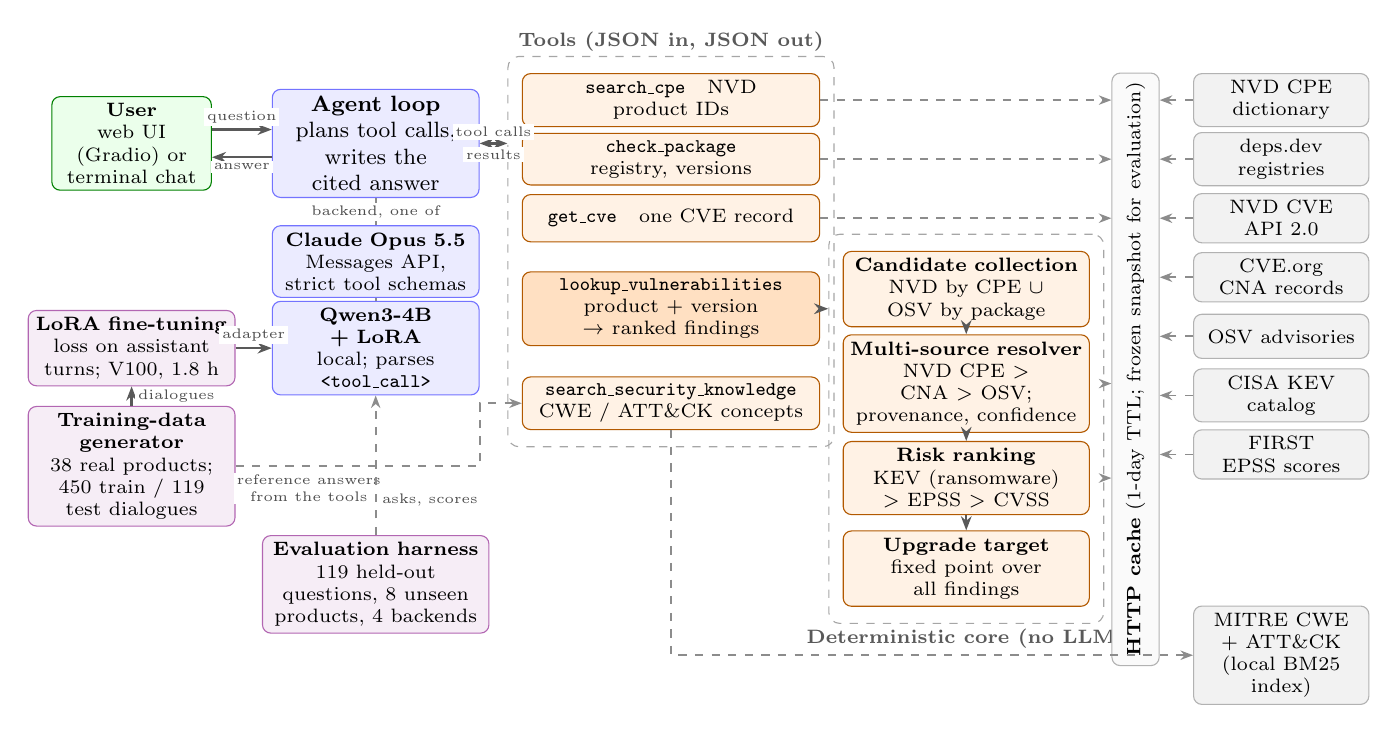
\begin{tikzpicture}[
    box/.style={draw=black!60, rounded corners=3pt, align=center, font=\scriptsize,
                minimum height=0.8cm, fill=white, inner sep=2.5pt,
                execute at begin node={\hyphenpenalty=10000\relax}},
    llm/.style={box, fill=blue!8, draw=blue!55, text width=2.45cm},
    tool/.style={box, fill=orange!10, draw=orange!70!black, minimum height=0.6cm, text width=3.6cm},
    core/.style={box, fill=orange!10, draw=orange!70!black, text width=2.95cm},
    data/.style={box, fill=gray!10, draw=gray!60, text width=2.05cm, minimum height=0.56cm},
    io/.style={box, fill=green!8, draw=green!50!black, text width=1.85cm},
    off/.style={box, fill=violet!7, draw=violet!60, text width=2.45cm},
    group/.style={draw=black!35, dashed, rounded corners=4pt, inner sep=5pt},
    glabel/.style={font=\scriptsize\bfseries, black!65, inner sep=1.5pt},
    arr/.style={-{Stealth[length=1.8mm]}, thick, black!65},
    darr/.style={-{Stealth[length=1.6mm]}, semithick, black!45, dashed},
    lbl/.style={font=\tiny, black!70, fill=white, inner sep=1pt},
]
% ---------------- user, agent and its two backends ----------------
\node[io]  (user)  at (0,0) {\textbf{User}\\web UI (Gradio) or terminal chat};
\node[llm, font=\footnotesize, minimum height=1.05cm] (agent) at (3.1,0)
      {\textbf{Agent loop}\\plans tool calls, writes the cited answer};
\node[llm] (claude) at (3.1,-1.5) {\textbf{Claude Opus 5.5}\\Messages API, strict tool schemas};
\node[llm] (qwen)   at (3.1,-2.6) {\textbf{Qwen3-4B + LoRA}\\local; parses \texttt{<tool\_call>}};
\draw[black!45, semithick] (agent.south) -- node[lbl]{backend, one of} (claude.north);
\draw[black!45, semithick] (claude.south) -- (qwen.north);

\draw[arr] ([yshift=5pt]user.east) -- node[lbl, above=1pt]{question} ([yshift=5pt]agent.west);
\draw[arr] ([yshift=-5pt]agent.west) -- node[lbl, below=1pt]{answer} ([yshift=-5pt]user.east);

% ---------------- tools ----------------
\node[tool] (t1) at (6.85, 0.55) {\texttt{search\_cpe}\quad NVD product IDs};
\node[tool] (t2) at (6.85,-0.2)  {\texttt{check\_package}\quad registry, versions};
\node[tool] (t4) at (6.85,-0.95) {\texttt{get\_cve}\quad one CVE record};
\node[tool, fill=orange!24] (t3) at (6.85,-2.1)
      {\texttt{lookup\_vulnerabilities}\\product + version $\rightarrow$ ranked findings};
\node[tool] (t5) at (6.85,-3.3) {\texttt{search\_security\_knowledge}\\CWE / ATT\&CK concepts};
\begin{scope}[on background layer]
  \node[group, fit=(t1)(t5), inner ysep=6pt] (tools) {};
\end{scope}
\node[glabel, anchor=south] at (tools.north) {Tools (JSON in, JSON out)};
\draw[arr, {Stealth[length=1.8mm]}-{Stealth[length=1.8mm]}] (agent.east) --
      node[lbl, above=1pt]{tool calls} node[lbl, below=1pt]{results} (agent.east -| tools.west);

% ---------------- deterministic core ----------------
\node[core] (c1) at (10.6,-1.85) {\textbf{Candidate collection}\\NVD by CPE $\cup$ OSV by package};
\node[core] (c2) at (10.6,-3.05) {\textbf{Multi-source resolver}\\NVD CPE $>$ CNA $>$ OSV;\\provenance, confidence};
\node[core] (c3) at (10.6,-4.25) {\textbf{Risk ranking}\\KEV (ransomware) $>$ EPSS $>$ CVSS};
\node[core] (c4) at (10.6,-5.4) {\textbf{Upgrade target}\\fixed point over all findings};
\draw[arr] (c1) -- (c2);
\draw[arr] (c2) -- (c3);
\draw[arr] (c3) -- (c4);
\begin{scope}[on background layer]
  \node[group, fit=(c1)(c4), inner ysep=6pt] (core) {};
\end{scope}
\node[glabel, anchor=north] at (core.south) {Deterministic core (no LLM)};
\draw[arr] (t3.east) -- (t3.east -| core.west);

% ---------------- cache and data sources ----------------
\node[draw=gray!60, fill=gray!4, rounded corners=3pt, minimum width=0.6cm, minimum height=5.35cm,
      anchor=north] (cache) at (12.75, 0.9)
      {\rotatebox{90}{\scriptsize \textbf{HTTP cache} (1-day TTL; frozen snapshot for evaluation)}};
\node[data] (s1) at (14.6, 0.55)  {NVD CPE dictionary};
\node[data] (s2) at (14.6,-0.2)   {deps.dev registries};
\node[data] (s3) at (14.6,-0.95)  {NVD CVE API 2.0};
\node[data] (s4) at (14.6,-1.7)   {CVE.org CNA records};
\node[data] (s5) at (14.6,-2.45)  {OSV advisories};
\node[data] (s6) at (14.6,-3.2)   {CISA KEV catalog};
\node[data] (s7) at (14.6,-3.95)  {FIRST EPSS scores};
\node[data, minimum height=0.8cm] (s8) at (14.6,-6.5) {MITRE CWE + ATT\&CK\\(local BM25 index)};
\foreach \s in {s1,s2,s3,s4,s5,s6,s7} { \draw[darr] (\s.west) -- (\s.west -| cache.east); }
\draw[darr] (t1.east) -- (t1.east -| cache.west);
\draw[darr] (t2.east) -- (t2.east -| cache.west);
\draw[darr] (t4.east) -- (t4.east -| cache.west);
\draw[darr] (core.east |- c2) -- (c2 -| cache.west);
\draw[darr] (core.east |- c3) -- (c3 -| cache.west);
\draw[darr] (t5.south) |- (s8.west);

% ---------------- offline: training data, fine-tuning, evaluation ----------------
\node[off] (lora) at (0,-2.6)  {\textbf{LoRA fine-tuning}\\loss on assistant turns; V100, 1.8 h};
\node[off] (gen)  at (0,-4.1)  {\textbf{Training-data generator}\\38 real products; 450 train / 119 test dialogues};
\node[off, text width=2.7cm] (eval) at (3.1,-5.6)
      {\textbf{Evaluation harness}\\119 held-out questions, 8 unseen products, 4 backends};
\draw[arr] (lora.east) -- node[lbl, above=1pt]{adapter} (qwen.west);
\draw[arr] (gen.north) -- node[lbl, right=1pt]{dialogues} (lora.south);
\draw[darr] (gen.east) -- node[lbl, below=2pt, pos=0.3, align=center]{reference answers\\from the tools}
      ([xshift=-10pt]gen.east -| tools.west) |- (t5.west);
\draw[darr] (eval.north) -- node[lbl, right=1pt, pos=0.25]{asks, scores} (qwen.south);
\end{tikzpicture}

\caption{Final system design. Blue: LLM components; orange: deterministic code; gray: external data, reached through an on-disk HTTP cache (dashed arrows); purple: offline data generation, fine-tuning and evaluation. The agent can run on Claude Opus 5.5 or on the LoRA-fine-tuned Qwen3-4B with the same prompt, tools and loop. \texttt{lookup\_vulnerabilities} wraps the deterministic core; the CWE/ATT\&CK index is built locally from MITRE's releases.}
\label{fig_system}
\end{figure*}

\section{Final System Design}
\label{sec:design}

Figure~\ref{fig_system} shows the implemented system. A user asks a question in the Gradio~\cite{abid2019gradio} web interface (Figure~\ref{fig_teaser}) or a terminal chat. The \textbf{agent loop} sends the conversation to the LLM backend with five tool schemas, executes the requested tools, returns their JSON results and repeats, up to ten steps, until the model answers. Each browser session has its own agent, so follow-up questions keep their context.

The two \textbf{backends} share the prompt, tools and loop. Claude Opus 5.5 is called through the Messages API with strict tool schemas (so arguments always match the schema) and prompt caching for the system prompt and tool definitions. The Qwen3-4B backend renders the conversation with the model's own chat template, generates greedily, and parses \texttt{<tool\_call>} blocks; malformed calls are returned to the model as tool errors rather than dropped.

The \textbf{tools} return compact JSON. \texttt{lookup\_vulnerabilities} returns counts, the upgrade target, CVEs the target still does not fix, the top 15 affected findings in full (status, source, confidence, evidence, fix version, KEV, EPSS, CVSS, reason and URLs) and the rest by ID. All external requests go through an \textbf{HTTP cache} with a one-day lifetime that also enforces NVD's rate limit; in evaluation mode it serves the cached snapshot regardless of age, so every run sees the same data. The \textbf{offline pipeline} generates training and test dialogues from the core, fine-tunes the adapter on a V100 and evaluates all backends on held-out questions.

Compared with the Phase 1 design, the fixed pipeline (query understanding, router, resolvers) became tools the model chooses among, because the right sequence depends on what the earlier calls return (\eg, a missing version or an ambiguous product). Version parsing, which Phase 1 assigned to the LLM, is done entirely in code. The planned 7--8B open model became a 4B one, for the training-memory reasons in Section~\ref{sec:ft}.

%-------------------------------------------------------------------------
\section{Methodology}
\label{sec:method}

\subsection{Validating the core}
Before building on the core we compared it with NVD's own server-side version matching (\texttt{virtualMatchString}) on six product-version pairs (Log4j 2.14.1 and 2.17.0, jackson-databind 2.9.8, requests 2.19.0, Django 3.2.0, lodash 4.17.15). The set of CVEs our resolver marks affected from NVD data equals NVD's result in all six. For the pre-release Log4j 2.0-beta9, ours is a strict superset, because NVD's matcher misses ranges whose lower bound is the release line; we treat this as an expected divergence. These checks and 55 offline unit tests are part of the repository.

\subsection{Data, split and snapshot}
\label{sec:data}
We chose 38 widely used libraries with substantial CVE histories, 15 Maven, 13 PyPI and 10 npm, and verified each one's CPE pairs, package name and CNA names by hand. Eight of them (SnakeYAML, Apache Shiro, H2, Werkzeug, Paramiko, lxml, Handlebars, ws) form the test set; no test product appears in training. For each product we sample twelve published versions, spread across its release history, and create one dialogue per version from varied question templates (``Is X 1.2.3 vulnerable?'', ``package-lock.json has X@1.2.3. Should we be worried?''). The dialogue contains the real tool calls (product verification, then lookup), their real outputs, and an answer rendered from the output by templates: a two-sentence summary, the top five findings with the reason for each rank and links, a list of the rest, undetermined CVEs, the remediation, and the data date. Three special cases per product teach abstention: no version given (ask for it), a version that was never published (say so and list the nearest published ones) and a misspelled package (say it was not found). This gives 450 training dialogues (360 lookups) and 119 test dialogues (96 lookups, 8 missing-version, 8 unpublished-version, 7 unknown-package). Dialogues are 3.5k tokens at the median and at most 13.3k. Test lookups have 7.0 affecting CVEs on average (up to 20), 7 have none, and 12 include advisories that exist only in OSV.

All data was retrieved on 2026-11-17 and frozen: the 650 cached responses (38\,MB) are the snapshot every evaluation runs on.

\subsection{Backends}
We compare four backends on the same questions:
(1) \textbf{Claude + tools}: Claude Opus 5.5, medium reasoning effort, the four lookup tools;
(2) \textbf{Claude, no tools}: the same model with a short prompt asking for the affecting CVEs in risk order, the exploited ones and the upgrade target, answered from its own knowledge;
(3) \textbf{Qwen3-4B base}: Qwen3-4B-Instruct-2507 with the tools and the full system prompt;
(4) \textbf{Qwen3-4B + LoRA}: the same with our adapter.
The conceptual-retrieval tool is left out of this evaluation so that the tool list matches the fine-tuning data.

\subsection{Fine-tuning}
\label{sec:ft}
We fine-tune Qwen3-4B-Instruct-2507 (Apache-2.0, native tool-call template, text-only) with LoRA~\cite{hu2022lora} on all linear layers (rank 16, $\alpha=32$, dropout 0.05; 33.0M trainable parameters, 0.81\%). The loss covers only assistant turns (tool calls and answers); system, user and tool messages are context, located by rendering each prefix with the chat template and checking that the template is prefix-stable. We train for two epochs with AdamW, learning rate $2\times10^{-4}$, cosine schedule with 5\% warm-up, one dialogue per forward pass and 8-step gradient accumulation (113 optimizer steps), fp16 weights with fp32 adapters and gradient checkpointing, on one 32\,GB V100 of Northeastern's Explorer cluster.

Two memory issues decided what fits. First, a 152k-token vocabulary makes full logits for a 13k-token dialogue cost over 8\,GB, so we apply the output layer only at the labelled positions. Second, on GPUs without FlashAttention, PyTorch's scaled dot-product attention falls back to the math kernel when grouped-query attention is requested, which materializes the full heads$\times L\times L$ attention matrix and ran out of memory; repeating the key/value heads instead lets the memory-efficient kernel run. With these changes training took 1\,h\,49\,min. We chose a 4B model over the planned 7--8B so that the longest (13k-token) dialogues train without truncation in 32\,GB. Each epoch was evaluated on the held-out test dialogues, and the run is logged to Weights \& Biases.

\subsection{Metrics}
\label{sec:metrics}
For lookup questions the reference is the core's output for that question: the affected and undetermined CVE sets, the top-ranked CVE, the KEV subset and the upgrade target. From each answer we extract vulnerability IDs (CVE and GitHub advisory IDs, mapping advisories to the CVE they alias) and compute: \textbf{called lookup}, whether the agent called \texttt{lookup\_vulnerabilities}; \textbf{CVE recall} and \textbf{precision} of the mentioned IDs against the affected set; \textbf{top CVE}, whether the first-ranked CVE is mentioned; \textbf{upgrade}, whether the reference upgrade target appears; \textbf{citation rate}, the fraction of mentioned IDs written as a link; and \textbf{clean}, for versions with no affecting CVE, whether the answer names none. An ID is \textbf{unsupported} if it is in neither the reference sets nor any tool result of that run. A special case is correct if the answer asks for the version, or says the package or version was not found, and names no CVE.

The scorer was audited by reading every answer it marked wrong in the Claude run. This found three scorer errors, all of which wrongly penalized correct answers: advisory IDs were not counted, a group shorthand (``CVE-2026-1064xx'') was read as an ID, and phrasings such as ``has never been released'' were not recognized as abstention. We fixed the scorer and re-scored all four saved runs; no model was re-run. We also checked every unsupported ID against NVD and OSV to see whether it exists.

\subsection{Conceptual questions}
We wrote 36 conceptual questions with the CWE or ATT\&CK entries that count as correct, 24 asked directly (``What is CWE-502?'', ``What is server-side request forgery?'') and 12 paraphrased so that they avoid the entry's name (``Someone typed \texttt{' OR 1=1 --} into our login form and got in. What class of bug is that?''). We measure retrieval alone (the question as the query; hit@1, hit@5, MRR) and Claude end to end with the retrieval tool versus from memory: whether the answer mentions an expected ID, whether it links that entry's official URL, and whether it mentions an ID that is not a current catalog entry (made up, deprecated or revoked).

%-------------------------------------------------------------------------
\section{Results}
\label{sec:results}

\begin{table}[t]
\centering
\footnotesize
\setlength{\tabcolsep}{3.2pt}
\begin{tabular}{@{}lcccc@{}}
\toprule
 & \multicolumn{2}{c}{Qwen3-4B} & \multicolumn{2}{c}{Claude Opus 5.5} \\
\cmidrule(lr){2-3}\cmidrule(l){4-5}
Metric & base & + LoRA & no tools & + tools \\
\midrule
\multicolumn{5}{@{}l}{\emph{Lookup questions (96)}} \\
Called lookup          & 55.2 & 96.9 & --   & \best{100} \\
CVE recall             & 44.1 & 93.4 & 61.9 & \best{99.8} \\
CVE precision          & 55.8 & 96.6 & 63.8 & \best{100} \\
Top-ranked CVE named   & 52.8 & 96.6 & 80.9 & \best{100} \\
Upgrade target correct & 68.2 & 96.5 & 16.5 & \best{100} \\
Citation rate          & 2.2  & \best{99.5} & 0.0 & 85.5 \\
Clean versions correct & \best{100} & \best{100} & 0.0 & \best{100} \\
\midrule
\multicolumn{5}{@{}l}{\emph{All questions (119)}} \\
Special cases correct (23) & 87.0 & 95.7 & 4.3 & \best{100} \\
Answers w/ unsupported IDs & 10.1 & \best{0.0} & 78.2 & \best{0.0} \\
Unsupported IDs (count)    & 13 & \best{0} & 380 & \best{0} \\
Tool-call errors (count)   & 82 & \best{0} & -- & \best{0} \\
Seconds per question       & 31.6 & 29.1 & 20.0 & 19.0 \\
Cost (USD, 119 questions)  & GPU & GPU & 4.70 & 6.76 \\
\bottomrule
\end{tabular}
\caption{Results on the 119 held-out questions (eight products unseen in training). Percentages unless marked. ``Clean'' covers the 7 lookups whose version has no affecting CVE. Qwen runs on one V100 (1\,h for all 119 questions).}
\label{tab:main}
\end{table}

\textbf{Tools versus memory.} Table~\ref{tab:main} shows the main results. With the tools, Claude Opus 5.5 recalls 99.8\% of the affecting CVEs with 100\% precision, always names the top-ranked one, gives the correct upgrade target in every answer that has one, handles all 23 special cases, and mentions no unsupported ID. Its only recall loss is one Handlebars answer that summarized three CVEs as ``CVE-2026-339xx''. The same model without tools recalls 61.9\% and gives the correct upgrade target in only 16.5\% of answers. It also names CVEs for every one of the seven clean versions, and it gets only one of the 23 special cases right: in 21 of the others it lists CVEs instead of asking for the version or noticing that the version or package does not exist.

\textbf{What the unsupported IDs are.} We checked all 380 unsupported IDs of Claude without tools against NVD and OSV: every one exists. 345 are real CVEs of the product asked about whose ranges exclude the asked version, and the other 35 belong to bundled or related components (mostly libxml2 CVEs attributed to lxml, which bundles it, and PyCrypto CVEs attributed to Paramiko or cryptography) or are advisories for other versions. The model without tools therefore does not invent identifiers; it does not know which version ranges apply, which is exactly the decision the core makes. The base Qwen3-4B's 13 unsupported mentions are different: they are 8 distinct IDs, of which one does not exist (\texttt{CVE-2023-12345}) and seven belong to unrelated products such as a Tenda router and an Intel network driver.

\begin{figure}[t]
\centering
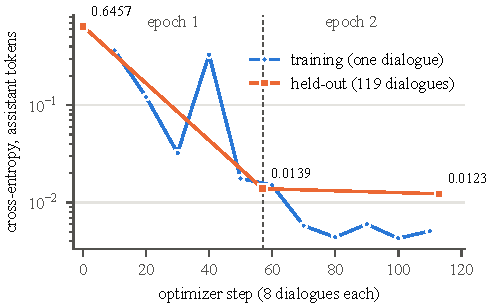
\includegraphics[width=\linewidth]{fig/loss_curve.pdf}
\caption{LoRA training on 450 dialogues. Held-out loss (token-weighted over the 119 test dialogues) falls from 0.646 to 0.014 in the first epoch and to 0.012 in the second. The training loss is that of a single dialogue per logged step and therefore noisy.}
\label{fig_loss}
\end{figure}

\textbf{Fine-tuning.} Figure~\ref{fig_loss} shows the training run. The held-out loss falls by a factor of 46 in the first epoch and changes little in the second, so two epochs were enough. In the agent evaluation (Table~\ref{tab:main}), the base Qwen3-4B fails in three ways: it skips the lookup in 43 of 96 questions, in the cases we read after misreading the \texttt{check\_package} result as ``version not found''; 82 of its lookup calls fail, 77 of them because required arguments (mostly the CNA names or CPE pairs) are missing, which a local model without schema enforcement can do; and it writes CVE IDs from memory. After fine-tuning it calls the lookup in 96.9\% of questions with no failed call, recall rises from 44.1\% to 93.4\% and precision from 55.8\% to 96.6\%, and no answer contains an unsupported ID. Its citation rate (99.5\%) is higher than Claude's (85.5\%) because it reproduces the training format, which links every ID. Its remaining errors are of three kinds. On Handlebars, whose versions have up to 20 affecting CVEs, it leaves out the same block of five consecutive IDs (CVE-2026-33937 to -33941) in ten answers, which accounts for most of its recall loss. In three lookups it asks for a version that was given, calls an existing version unpublished, or answers without the lookup. And once it answers ``no known CVEs'' for a version that does not exist; this is the most harmful kind of error, because it sounds like a clean result.

\begin{table}[t]
\centering
\footnotesize
\setlength{\tabcolsep}{4pt}
\begin{tabular}{@{}lccc@{}}
\toprule
\multicolumn{4}{@{}l}{\emph{(a) Retrieval alone, question as query}} \\
 & hit@1 & hit@5 & MRR \\
\midrule
Direct (24)      & 79.2 & 95.8 & 0.875 \\
Paraphrased (12) & 41.7 & 58.3 & 0.461 \\
All (36)         & 66.7 & 83.3 & 0.737 \\
\midrule
\multicolumn{4}{@{}l}{\emph{(b) Claude Opus 5.5 answers (36)}} \\
 & memory & + retrieval & \\
\midrule
Mentions expected ID      & 97.2 & \best{100} & \\
Links expected entry      & 5.6  & \best{100} & \\
Mentions non-current ID   & 2.8  & \best{0.0} & \\
Seconds / cost per answer & 10.1 / \$0.018 & 12.8 / \$0.030 & \\
\bottomrule
\end{tabular}
\caption{Conceptual questions about CWE weaknesses and ATT\&CK techniques. With retrieval, the agent rewrites paraphrased questions into the right query, so its end-to-end results are perfect on both question types although lexical retrieval alone misses most paraphrases.}
\label{tab:concept}
\end{table}

\textbf{Conceptual questions.} Table~\ref{tab:concept} shows that BM25 alone finds the right entry first for 79\% of direct but only 42\% of paraphrased questions: ``\texttt{' OR 1=1 --}'' shares no word with ``SQL injection''. End to end, the agent closes this gap: Claude names the concept first and searches for it (``SQL injection''), so it cites the expected entry in all 36 answers, paraphrased or not. From memory, Claude names the right ID almost as often (97.2\%) but links the official entry in only 2 of 36 answers. Its one non-current ID is instructive: for encoded PowerShell it cited T1562.001, which MITRE revoked in April 2026 and replaced with T1685; with retrieval the agent cites the current entry.

\textbf{Cost and latency.} With tools, Claude used 2.8 tool calls and \$0.057 per question on average (19\,s). The tool results add input tokens, so the no-tools run was cheaper (\$0.040 per question), but most of its answers were wrong. The fine-tuned 4B model answers in 29\,s on a V100 at no API cost, using 2.6 tool calls per question.

%-------------------------------------------------------------------------
\section{Discussion}
\label{sec:discussion}

\textbf{Divide the work by whether there is a right answer.} The no-tools baseline isolates where an LLM alone fails. Claude without tools knows the products' vulnerability histories well, and every ID it named exists. What it cannot do is decide range membership for a specific version, keep up with CVEs published after its training, or know that a version was never released. These are computations and lookups with a right answer, and moving them into code raised recall from 61.9\% to 99.8\% and upgrade correctness from 16.5\% to 100\%. The LLM remains essential for what code does poorly: understanding varied questions, choosing which product a name refers to, deciding when to ask instead of answering, and explaining the ranking.

\textbf{Deterministic data makes small-model fine-tuning cheap and safe.} Generating the training dialogues from the core gave labels that are correct by construction, cost nothing beyond API calls to public databases, and use no LLM output. Because the facts in every answer come from tool results, the adapter has nothing to memorize except the workflow, and the test products show that it generalizes to products it never saw. The small model still differs from the large one in completeness and judgement: it drops part of a long list, and some of its errors are about when to look something up or abstain, not about the facts it reports.

\textbf{Strict schemas matter for small models.} 82 of the base model's tool calls failed only because arguments were missing. Claude's API enforces the schema; the local model had to learn it. Constrained decoding would likely remove most of these failures even without fine-tuning, and is a cheap next step.

\textbf{Retrieval is mainly about verifiability and freshness.} For common weakness classes the large model already knows the right CWE, so retrieval changes little in correctness but turns 2 linked answers into 36, and it catches catalog changes such as the revoked T1562.001. Simple lexical retrieval was sufficient because the agent writes the query.

\textbf{Audit the scorer as carefully as the model.} All three scorer errors we found penalized correct answers in ways that would have understated the strongest system (\eg, recall 96.3\% instead of 99.8\%). Reading every failed answer, keeping raw outputs and re-scoring all runs with the same rules made the comparison fair without re-running any model.

%-------------------------------------------------------------------------
\section{Limitations}
\label{sec:limitations}

\textbf{Reference answers come from our own core.} Recall and precision measure agreement with the deterministic core, not with an independent ground truth. The core matched NVD's server-side matching on the six pairs we checked, but it inherits errors in NVD, CNA and OSV data, and CVEs without version data are reported as undetermined rather than resolved.

\textbf{Scale and coverage of the test set.} The test set has 119 questions about eight libraries in three ecosystems. None of the test products' affecting CVEs is in the KEV catalog, so the evaluation does not exercise KEV-first ranking on unseen products (58 training dialogues do). Each configuration was run once, with one fine-tuning seed and greedy decoding, so we report no variance.

\textbf{Template-shaped training data.} The training answers follow a small set of templates, which explains the low training loss and the uniform answer format of the fine-tuned model. It was not trained on multi-product questions, dependency files, follow-up turns or conceptual questions, and its abstention behaviour is learned from 90 dialogues.

\textbf{Links for OSV-only advisories.} Our tool gave advisory IDs that exist only in OSV (\eg, GHSA-\dots) an NVD URL, where they have no page. The training templates copied it, so the fine-tuned model wrote 48 such dead links; Claude used the OSV evidence links instead. We fixed the tool after the evaluation but did not retrain the adapter. The citation-rate metric checks that an ID is linked, not that the link resolves.

\textbf{Baseline and prompts.} The no-tools baseline uses a shorter prompt that does not ask the model to request missing versions, so its special-case score partly reflects the prompt. The comparison measures the model without our system rather than a prompt-matched ablation.

\textbf{Scope.} VulnScout covers open-source libraries with CPE or package identifiers. It does not scan lock files, container images or operating-system packages, and it inherits public databases' latency: a CVE not yet in NVD or OSV is invisible to it. Answers about exploitation rely on KEV and EPSS, which can lag real-world activity.

{\small
\bibliographystyle{ieee_fullname}
\bibliography{egbib}
}

\end{document}
